\documentclass{beamer}
 
\usepackage{beamerthemesplit}
\usepackage[utf8]{inputenc} 
\usepackage[russian]{babel}
\usepackage{amsmath,amssymb}
\usepackage{graphicx}
\usepackage{subfigure}
\usepackage{amsthm}
 
\renewcommand{\baselinestretch}{0.9}
 
\newtheorem{thm}{Теорема}
\newtheorem{lem}[thm]{Лемма}
\newtheorem{defn}{Определение}
\newtheorem{exmpr}{Использование в R}
\newtheorem{exmp}{Пример}

\date{\today}
 
\begin{document}
\title[\hspace{15em}\insertframenumber/\inserttotalframenumber]{Лекция 2. Линейные модели.}
\begin{frame}
  \titlepage
\end{frame}
 
 
\begin{frame}[containsverbatim]
\frametitle{Простая линейная регрессия}
\begin{defn}
$$y = b_0+b_1x_1+\ldots+b_px_p+\epsilon$$
\end{defn}
\begin{exmpr}
\begin{verbatim}
> library(faraway)
> (lm1<-lm(Species~Area+Elevation+Nearest+Scruz+Adjacent,
data=gala))
Call:
lm(formula = Species ~ Area + Elevation + Nearest + 
Scruz + Adjacent,data = gala)
Coefficients:
(Intercept)      Area  Elevation   Nearest      Scruz  
   7.068221 -0.023938   0.319465  0.009144  -0.240524  
   Adjacent  
  -0.074805
\end{verbatim}
\end{exmpr}
\end{frame}
 
\begin{frame}
\frametitle{Summary часть 1}
\begin{thm}
Если, 
$\epsilon\sim\mathrm{N}(0,\sigma^2I)$, $\hat{b}$ - оценка, полученная методом наименьших квадратов, то\\
1) $\hat{b}\sim\mathrm{N}(b,(X^TX)^{-1}\sigma^2)$\\
2) $\hat{\sigma}^2 = \frac{\hat{\epsilon}^T\hat{\epsilon}}{n-p}$ - несмещенная оценка $\sigma^2$
\end{thm}
\begin{defn}[Стандартная ошибка]
Стандартная ошибка статистики - стандартное отклонение ее распределения.\\
Для $\hat{b}_i$: $se(\hat{b}_{i-1})=\sqrt{(X^TX)^{-1}_{ii}}\hat{\sigma}$
\end{defn}
\begin{defn}[t-статистика для одного предиктора]
$$t_i=\frac{\hat{b}_i}{se(\hat{b}_i)}\sim t(n-p)$$
Гипотеза: равенсто 0 предиктора.
\end{defn}

\end{frame}
 
\begin{frame}[containsverbatim]
\frametitle{Summary часть 1}
\begin{verbatim}
> summary(lm1)
Call:
lm(formula = Species ~ Area + Elevation + Nearest + Scruz + Adjacent, 
    data = gala)
Residuals:
     Min       1Q   Median       3Q      Max 
-111.679  -34.898   -7.862   33.460  182.584 
Coefficients:
             Estimate Std. Error t value Pr(>|t|)    
(Intercept)  7.068221  19.154198   0.369 0.715351    
Area        -0.023938   0.022422  -1.068 0.296318    
Elevation    0.319465   0.053663   5.953 3.82e-06 ***
Nearest      0.009144   1.054136   0.009 0.993151    
Scruz       -0.240524   0.215402  -1.117 0.275208    
Adjacent    -0.074805   0.017700  -4.226 0.000297 ***
---
Signif.codes: 0‘***’0.001‘**’0.01‘*’0.05‘.’0.1‘ ’1 
\end{verbatim}

\end{frame}

\begin{frame}[containsverbatim]
\frametitle{Summary часть 2}
\begin{verbatim}
Residual standard error: 60.98 on 24 degrees of freedom
Multiple R-squared: 0.7658,	Adjusted R-squared: 0.7171 
F-statistic:  15.7 on 5 and 24 DF,  p-value: 6.838e-07 
\end{verbatim}
\begin{defn}
$$R^2=1-\frac{\sum(\hat{y}_i-y_i)^2}{\sum(y_i-\overline{y})^2},\;\;\;\;\; R^2_{adj}=1-(1-R^2)\frac{n-1}{n-p}$$
$$F=\frac{(\sum(y_i-\overline{y})^2-\hat{\epsilon}^T\hat{\epsilon})/(p-1)}{(\hat{\epsilon}^T\hat{\epsilon})/(n-p)}\sim F(p-1,n-p)$$
Гипотеза: равенсто 0 всех предикторов.
\end{defn}
\end{frame}

\begin{frame}[containsverbatim]
\frametitle{Доверительные интервалы для коэффициентов}
\begin{exmpr}
\begin{verbatim}
> confint(lm1)
                  2.5 %      97.5 %
(Intercept) -32.4641006 46.60054205
Area         -0.0702158  0.02233912
Elevation     0.2087102  0.43021935
Nearest      -2.1664857  2.18477363
Scruz        -0.6850926  0.20404416
Adjacent     -0.1113362 -0.03827344
\end{verbatim}
\end{exmpr}
\end{frame}

\begin{frame}[containsverbatim]
\frametitle{Plot}
\begin{verbatim}
> plot(lm1)
\end{verbatim}
\begin{center}
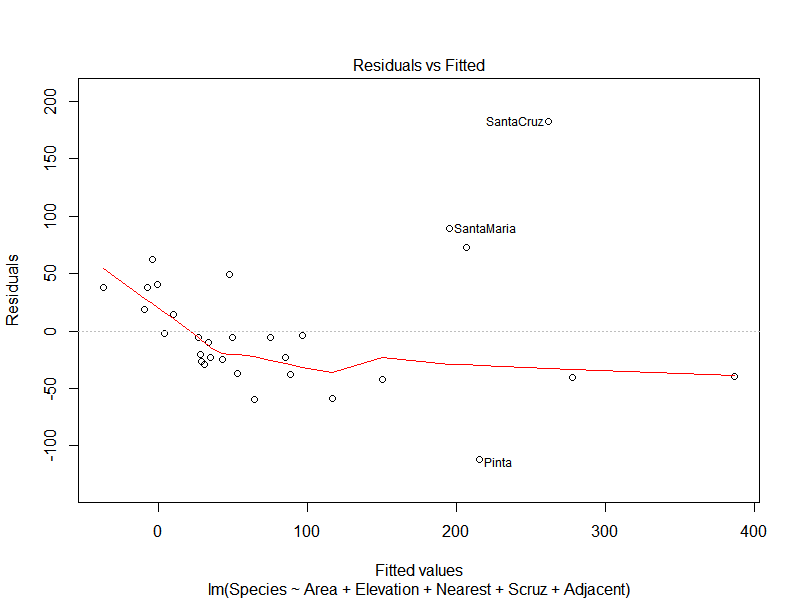
\includegraphics[width=1\textwidth,height=0.7\textheight]{lmplot1.png}
\end{center}

\end{frame}

\begin{frame}
\frametitle{Plot}
\begin{center}
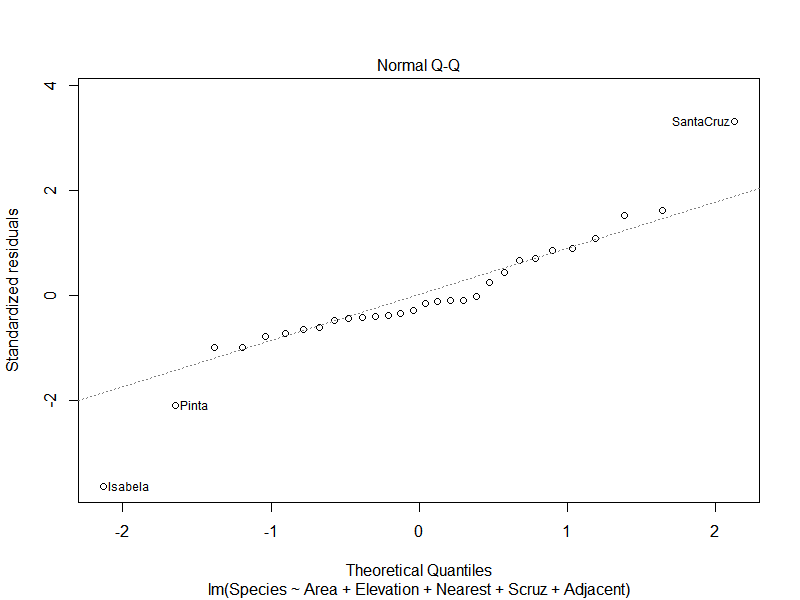
\includegraphics[width=1\textwidth,height=0.8\textheight]{lmplot2.png}
\end{center}
\end{frame}

\begin{frame}
\frametitle{Plot}
\begin{center}
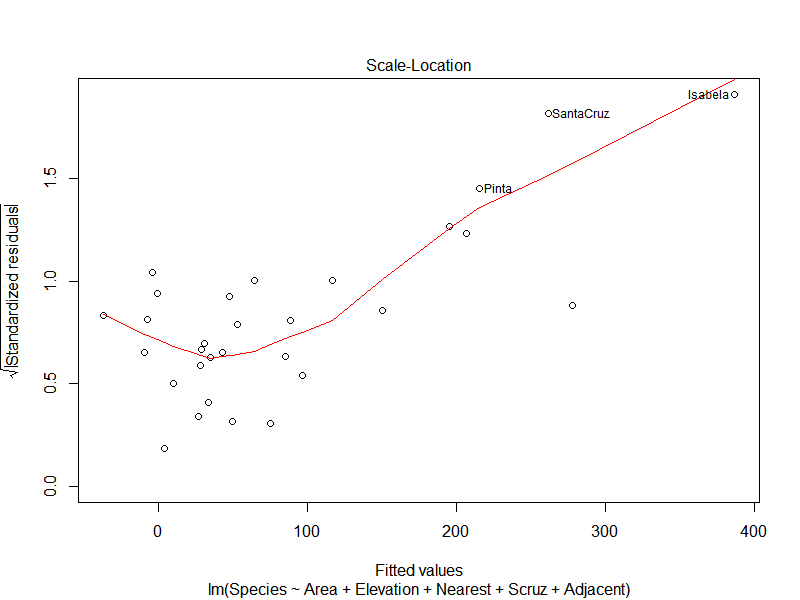
\includegraphics[width=1\textwidth,height=0.8\textheight]{lmplot3.png}
\end{center}
\end{frame}

\begin{frame}
\frametitle{Plot}
\begin{center}
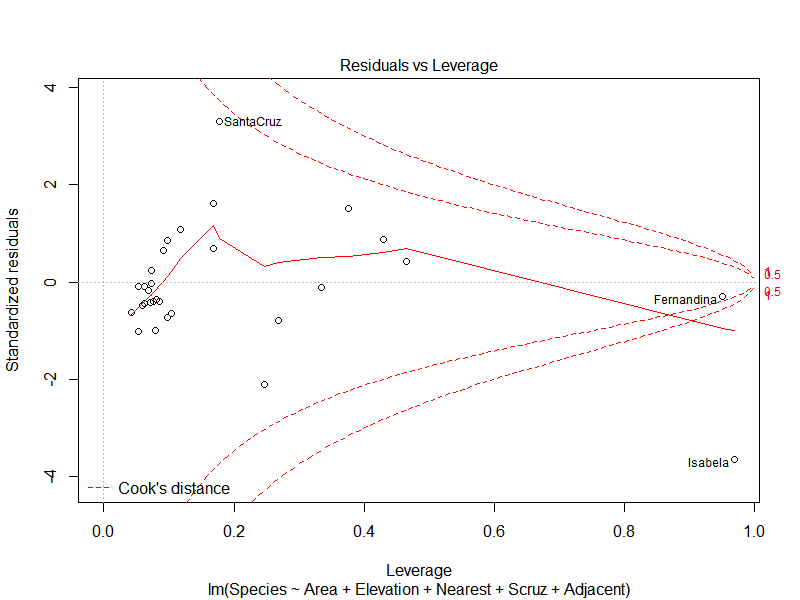
\includegraphics[width=1\textwidth,height=0.8\textheight]{lmplot4.png}
\end{center}
\end{frame}

\begin{frame}[containsverbatim]
\frametitle{Критерий Дарбина-Уотсона}
\begin{defn}[Статистика Дарбина-Уотсона]
$$DW=\dfrac{\sum\limits_{t=2}^p(\hat{\epsilon}_t-\hat{\epsilon}_{t-1})^2}{\sum\limits^p_{t=1}\hat{\epsilon}_t^2}$$
Используется для проверки автокорреляции остатков
\end{defn}
\begin{exmpr}
\begin{verbatim}
> library(lmtest)
> dwtest(lm1)
	Durbin-Watson test
data:  lm1 
DW = 2.4759, p-value = 0.9017
alternative hypothesis: true autocorrelation 
is greater than 0 
\end{verbatim}
\end{exmpr}
\end{frame}

\begin{frame}[containsverbatim]
\frametitle{Линейная регрессия без нулевого коэффициента}
\begin{defn}
$$y = b_1x_1+\ldots+b_px_p+\epsilon$$
\end{defn}
\begin{exmpr}
\begin{verbatim}
> lm(Species~Area+Elevation+Nearest+Scruz+Adjacent+0,
data=gala)
Call:
lm(formula = Species ~ Area + Elevation + Nearest + 
    Scruz + Adjacent + 0, data = gala)
Coefficients:
     Area  Elevation    Nearest      Scruz   Adjacent  
 -0.02664    0.33065    0.02590   -0.21359   -0.07646
\end{verbatim}
\end{exmpr}

\end{frame}

\begin{frame}[containsverbatim]
\frametitle{Линейная регрессия с пересечением}
\begin{defn}
$$y = b_0+b_1x_1+b_2x_2+b_3x_1x_2+\epsilon$$
\end{defn}
\begin{exmpr}
\begin{verbatim}
> lm(Species~Elevation*Adjacent,
data=gala)
Call:
lm(formula = Species ~ Elevation * Adjacent, data = gala)
Coefficients:
       (Intercept)           Elevation            Adjacent  
        -7.067e+00           2.908e-01          -5.780e-03  
Elevation:Adjacent  
        -4.633e-05  
\end{verbatim}
\end{exmpr}

\end{frame}


\begin{frame}[containsverbatim]
\frametitle{Линейная регрессия с пересечением}
\begin{defn}
$$y = b_0+b_1x_1+b_2x_2+b_3x_1x_2+\epsilon$$
\end{defn}
\begin{exmpr}
\begin{verbatim}
> lm(Species~Elevation+Adjacent+Elevation:Adjacent,
data=gala)
Call:
lm(formula = Species ~ Elevation + Adjacent + 
   Elevation:Adjacent, data = gala)
Coefficients:
       (Intercept)           Elevation            Adjacent  
        -7.067e+00           2.908e-01          -5.780e-03  
Elevation:Adjacent  
        -4.633e-05  
\end{verbatim}
\end{exmpr}

\end{frame}

\begin{frame}[containsverbatim]
\frametitle{Преобразование данных. Метод Бокса-Кокса}
\begin{defn}
Хотим преобразовать вектор $y$ в $g_{\lambda}(y)$,
$$g_{\lambda}(y)=\begin{cases}
 \frac{y^{\lambda}-1}{\lambda} & \lambda \ne 0 \\
 \ln(y) & \lambda = 0
 \end{cases}$$
таким образом, чтобы максимизировать функцию правдоподобия.
\end{defn}
\begin{columns}
\column{0.5\textwidth}
\begin{exmpr}
\begin{verbatim}
> library(MASS)
> bc <- boxcox(lm1,plot=T)
> m <- which.max(bc$y)
> lambda <- bc$x[m]
\end{verbatim}
\end{exmpr}
\column{0.5\textwidth}
\begin{center}
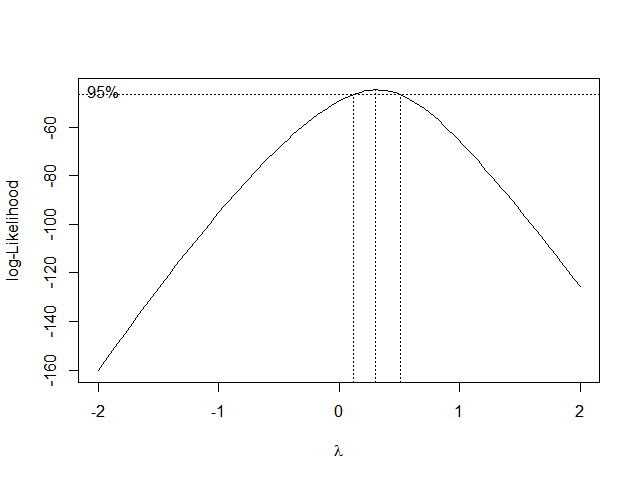
\includegraphics[width=1\textwidth,height=0.4\textheight]{boxcox.png}
\end{center}
\end{columns}
\end{frame}


\begin{frame}[containsverbatim]
\frametitle{Выбор параметров: функция step}
\begin{defn}[AIC и BIC]
$$AIC=2p-2\ln(L),\;\;\;\;\;BIC=\ln(n)-2\ln(L)$$
где L - значение функции правдоподобия.
\end{defn}
\begin{exmpr}
\begin{verbatim}
Start:  AIC=251.93
Species ~ Area + Elevation + Nearest + Scruz + Adjacent
            Df Sum of Sq    RSS    AIC
- Nearest    1         0  89232 249.93
- Area       1      4238  93469 251.33
- Scruz      1      4636  93867 251.45
<none>                    89231 251.93
- Adjacent   1     66406 155638 266.62
- Elevation  1    131767 220998 277.14
\end{verbatim}
\end{exmpr}

\end{frame}

\begin{frame}[containsverbatim]
\frametitle{Выбор параметров: функция step}

\begin{exmpr}
\begin{verbatim}
Step:  AIC=249.93
Species ~ Area + Elevation + Scruz + Adjacent

            Df Sum of Sq    RSS    AIC
- Area       1      4436  93667 249.39
<none>                    89232 249.93
- Scruz      1      7544  96776 250.37
- Adjacent   1     72312 161544 265.74
- Elevation  1    139445 228677 276.17
Step:  AIC=249.39
Species ~ Elevation + Scruz + Adjacent
\end{verbatim}
\end{exmpr}

\end{frame}

\begin{frame}[containsverbatim]
\frametitle{Выбор параметров: функция step}

\begin{exmpr}
\begin{verbatim}
            Df Sum of Sq    RSS    AIC
- Scruz      1      6336 100003 249.35
<none>                    93667 249.39
- Adjacent   1     69860 163527 264.11
- Elevation  1    275784 369451 288.56
Step:  AIC=249.35
Species ~ Elevation + Adjacent
            Df Sum of Sq    RSS    AIC
<none>                   100003 249.35
- Adjacent   1     73251 173254 263.84
- Elevation  1    280817 380820 287.47
Call:
lm(formula = Species ~ Elevation + Adjacent, data = gala)
Coefficients:
(Intercept)    Elevation     Adjacent  
    1.43287      0.27657     -0.06889  
\end{verbatim}
\end{exmpr}

\end{frame}

\begin{frame}[containsverbatim]
\frametitle{Предсказание новых значений}
\begin{exmpr}
\begin{verbatim}
> lm3<-lm(Species~Elevation+Adjacent,data=gala)
> preds <- data.frame(Elevation=400, Adjacent=300)
> predict(lm3, newdata=preds) 
       1 
91.39454
> predict(lm3, newdata=preds, interval="confidence")
       fit      lwr     upr
1 91.39454 68.52808 114.261
\end{verbatim}
\end{exmpr}

\end{frame}


\end{document}